\documentclass[11pt, a4paper, oneside]{scrartcl}
\usepackage[hidelinks]{hyperref}
\usepackage{polski}
\usepackage[utf8]{inputenc}

\usepackage{amssymb}
\usepackage{amsmath}
\usepackage[pdftex]{graphicx}
\usepackage[margin=2.5cm]{geometry}

\usepackage{algorithm2e}
\usepackage{algorithmic}
\usepackage{mathtools}
\usepackage{multirow}
\usepackage{pbox}
\usepackage{hyperref}
\usepackage{tikz}
\usepackage{tkz-euclide}
\usetkzobj{all} 
\usepackage{array}
\usepackage{float}

\begin{document}


\begin{titlepage}

\centering
    \vfill
    {\bfseries\Large
        Wydział Matematyki i Nauk Informacyjnych
    }    
    \vfill
	
\includegraphics[scale=0.2]{logo_mini.png}
	\vfill
	{\bfseries\Large
        Dokumentacja projektu \\
	Grafika 3D -- ,,Iluminacje świąteczne''
    } 
\vfill
	{
	\textbf{Jadwiga Słowik}
	}
 \vfill
{
     Wersja 1.0 \\ 
     \today
}
\end{titlepage}

\tableofcontents
\newpage

\section{Specyfikacja}
\subsection{Opis biznesowy}
Niniejsza aplikacja zawiera trójwymiarową scenę 3D przedstawiającą fragment parku z~choinkami w~nocy.
Ów park jest ozdobiony ,,iluminacjami'' świątecznymi. Są to kolorowe lampki ułożone we~wzory, oświetlające całą scenę.
Na~gruncie widoczne są rozbłyski owych lampek. 

Na~scenie znajduje~się również obiekt (turkusowy kot), którym~użytkownik może sterować w~czterech kierunkach. Ponadto, użytkownik może patrzeć na~scenę przy~pomocy jednej z~trzech kamer:
\begin{itemize}
	\item Kamera nieruchoma, patrząca na~całą scenę
	\item Kamera nieruchoma, śledząca kota
	\item Kamera ruchoma -- patrząca ,,oczami'' kota
\end{itemize}
oraz~zapewniony jest wybór jednego z~trzech dostępnych modeli cieniowania:
\begin{itemize}
	\item Cieniowanie Gorauda
	\item Cieniowanie Phonga
	\item Cieniowanie płaskie
\end{itemize}
i~wybór jednego z~dwóch modeli oświetlenia:
\begin{itemize}
	\item Oświetlenie Phonga
	\item Oświetlenie Blinna
\end{itemize}

\subsection{Wymaganie funkcjonalne}
Na~poniższym diagramie przedstawiono zbiór przypadków użycia dla~użytkowanika: \\
\begin{figure}[H]
	\centering 
	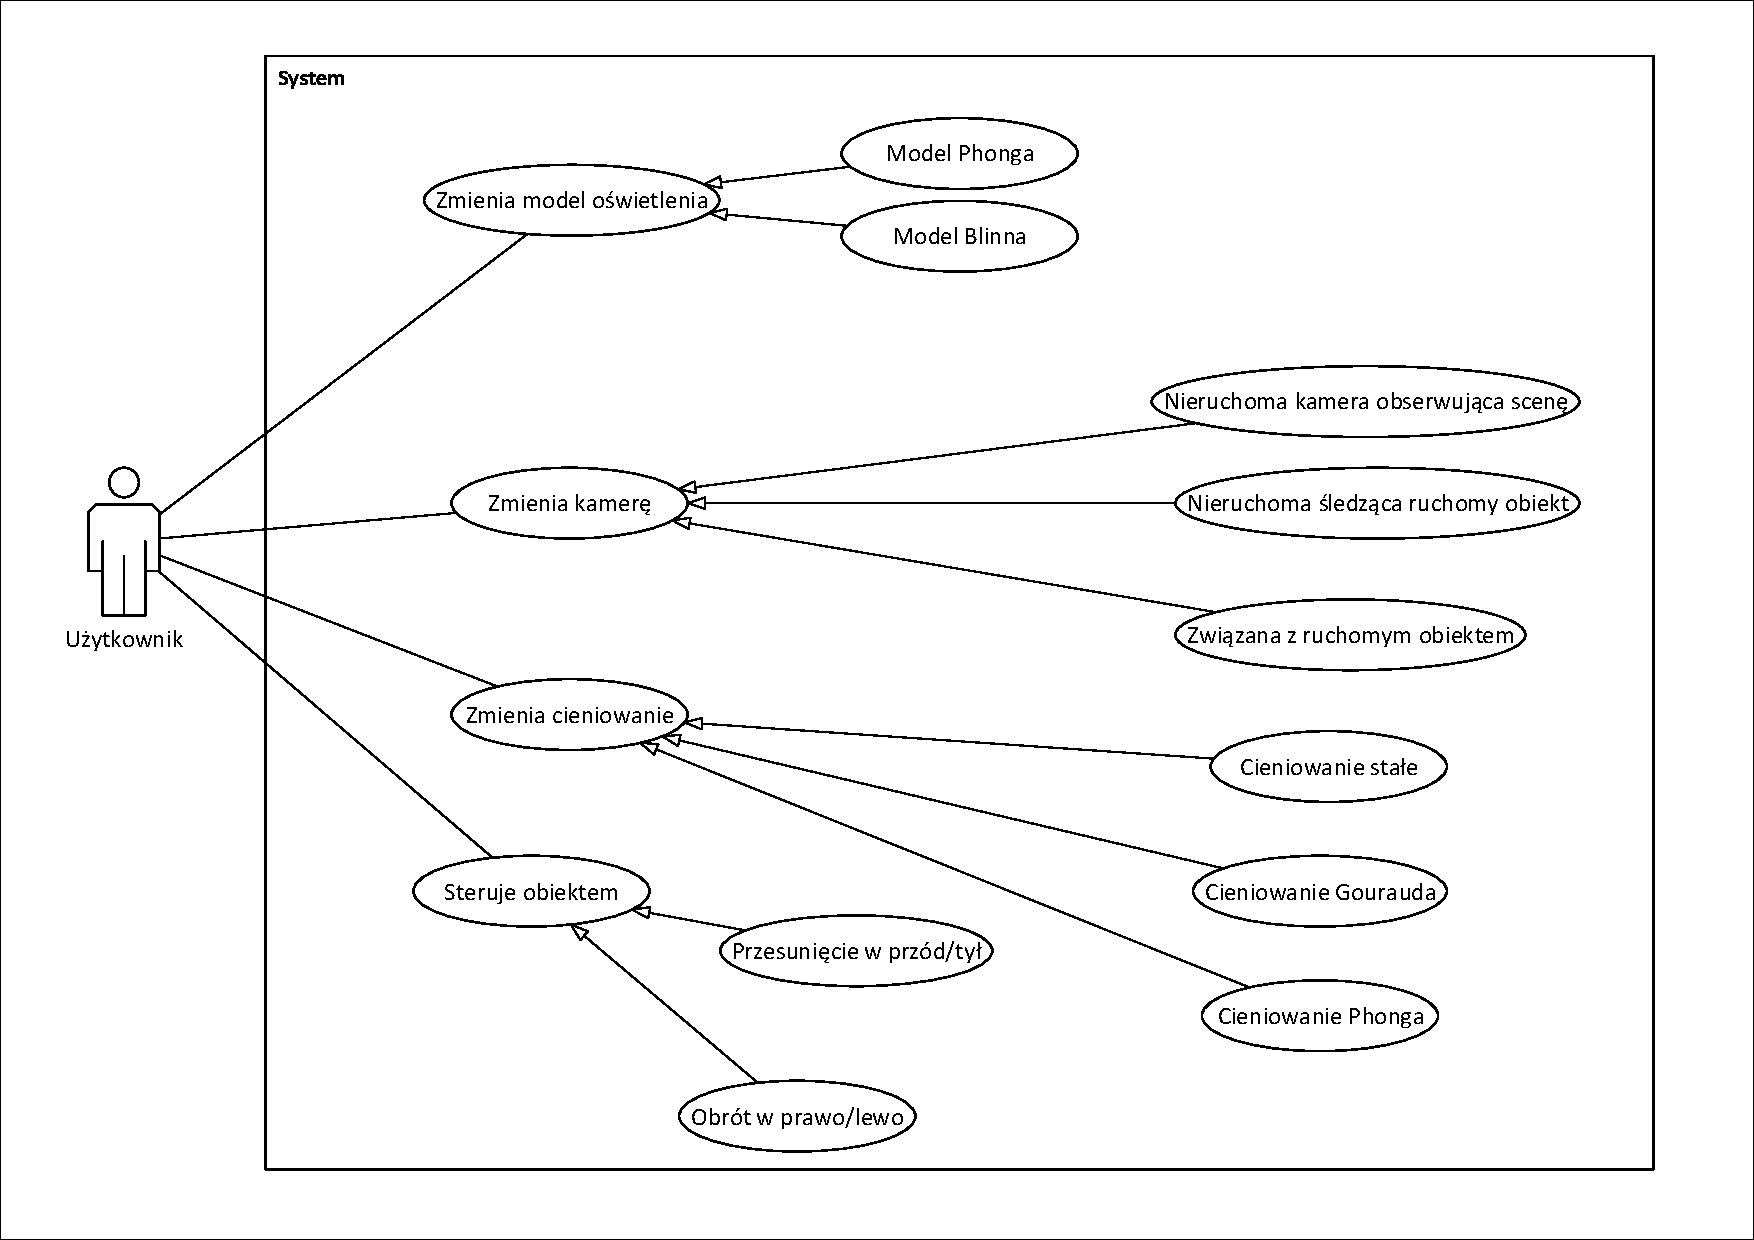
\includegraphics[scale=0.5]{UseCase.pdf}
\end{figure}
Opisy przypadków użycia dla~użytkownika: \\ \\
\begin{tabular}{|m{2.5cm}|m{3cm}|m{5cm}|m{5cm}|}
	\hline
	\textbf{Aktor} & \textbf{Nazwa} & \textbf{Opis} & \textbf{Odpowiedź systemu} \cr
	\hline
Użytkownik     	    &  Zmienia model oświetlenia & Zmiania algorytm obliczania koloru światła dla~pixela & Nieznaczna zmiana wyglądu rysowania sceny \cr
	\hline
			    & Zmienia kamerę na~nieruchomą obserwującą scenę & Zmiana sposobu patrzenia na~scenę & Zmiana obrazu widzianego przez~użytkownika na~obraz całej sceny \cr
	\hline
			   & Zmienia kamerę na~nieruchomomą śledzącą ruchomy obiekt &  Zmiana sposobu patrzenia na~scenę & Zmiana obrazu widzianego przez~użytkownika. Wraz ze~zmianą położenia kota, ulega również zmianie obraz widziany na~ekranie, ale kamera nie~zmienia położenia. \cr
	\hline
			   & Zmienia kamerę na~ruchomą związaną z~ruchomym obiektem & Zmiana sposobu patrzenia na~scenę & Zmiana obrazu widzianego przez~użytkownika. Na~ekranie przedstawiony jest obraz widziany ,,oczami'' obiektu ruchomego. Ów~obraz zmienia~się po~zmianie położenia obiektu ruchomego \cr
	\hline
			& Zmienia cieniowanie & Zmienia sposób cieniowania na~jeden z trzech możliwych (cieniowanie Phonga, Gorauda, płaskie) & Zmiana wyglądu sceny \cr
	\hline
			& Steruje obiektem & Steruje obiektem (w~jednym z~trzech kierunków) & Zmiana położenia / ustawienia ruchomego obiektu \cr
	\hline
\end{tabular}

\subsection{Harmonogram projektu}
\begin{tabular}{|m{0.5cm}|m{5cm}|m{2.5cm}|m{2.5cm}|m{2.5cm}|}
	\hline
\textbf{Nr} & \textbf{Zadanie} & \textbf{Data rozpoczęcia} & \textbf{Data zakończenia} & \textbf{Przeznaczony czas} \cr
	\hline
$1$ & Wstępna analiza zadania & 5.12.2016 & 18.12.2016 & 12 dni \cr
	\hline
$2$ & Przygotowanie specyfikacji & 18.12.2016 & 28.12.2016 & 1 dzień \cr
	\hline
$3$ & Wdrożenie technologii &  28.12.2016 & 28.01.2017 & 31 dni \cr
	\hline
$4$ & Projektowanie rozwiązania & 28.01.2017 & 06.02.2017 & 9 dni \cr
	\hline
$5$ & Implementacja & 06.02.2017 & 20.02.2017 & 14 dni \cr
	\hline
$6$ & Przygotowanie końcowej dokumentacji & 20.02.2017 & 22.02.2017 & 2 dni \cr
	\hline
$7$ & Oddanie projektu & 22.02.2017 & 22.02.2017 & 1 dzień \cr
	\hline
\end{tabular}

\subsection{Architektura rozwiązania}
Rozwiązanie zostało podzielone na~poszczególne częsci:
\subsubsection{Rysowanie}
Do~rysowania przeznaczone są klasy pochodne klasy \textit{Drawer}. Implementują one konkretny algorytm, korzystając z~publicznych pól
obiektu, który~ma być rysowany (\textit{SceneActor}). 
\begin{figure}[H]
	\centering 
	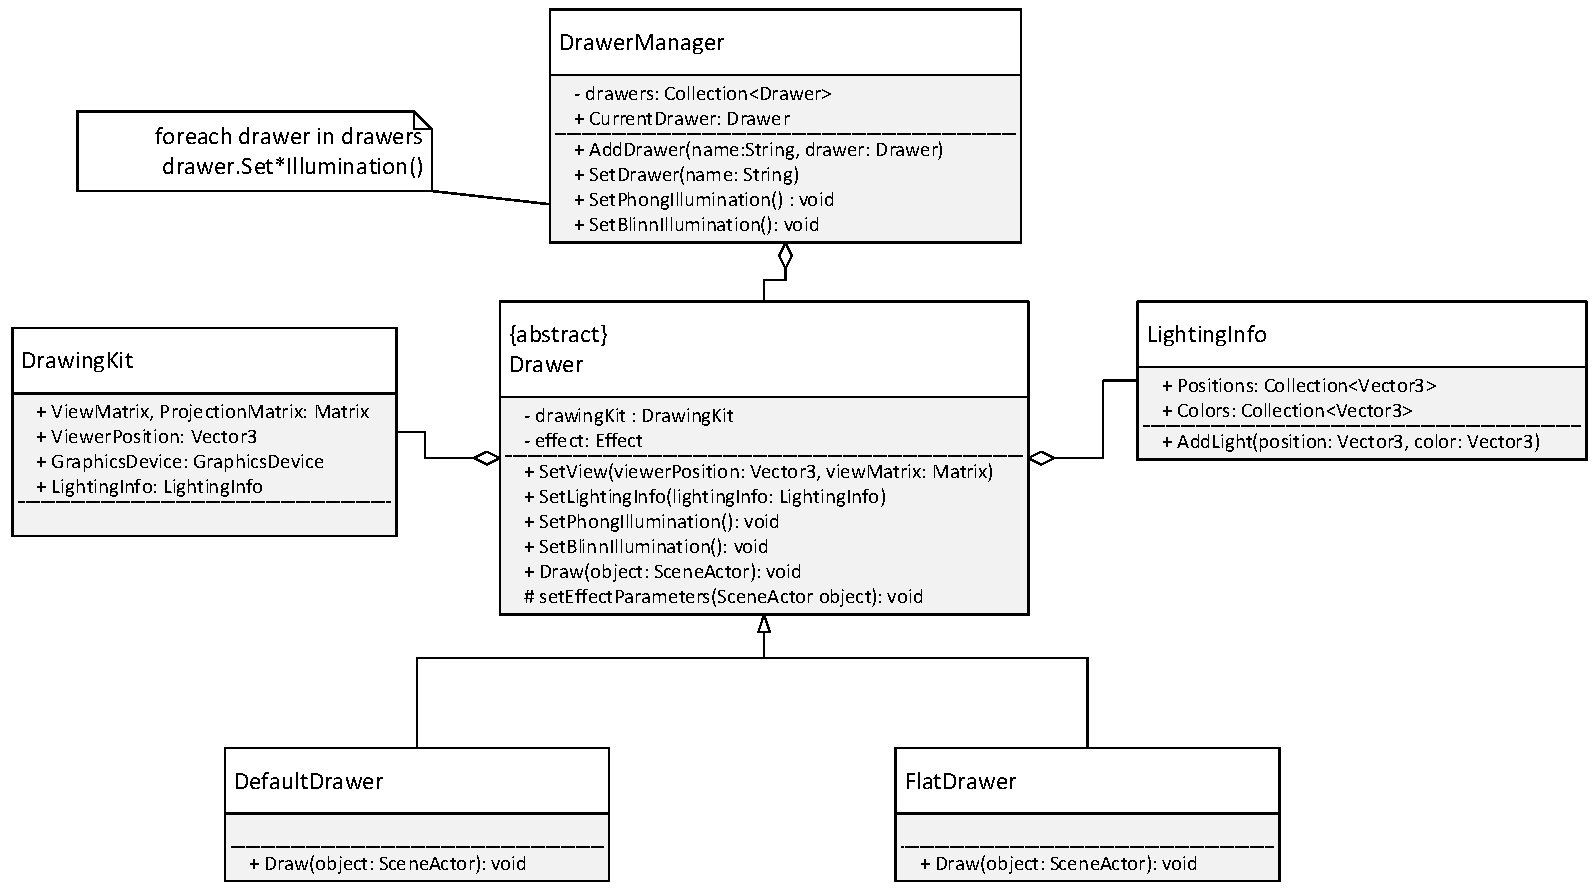
\includegraphics[scale=0.6]{Drawers.pdf}
\end{figure}
Każdy ,,rysownik'' posiada ,,przybornik do rysowania'' (\textit{DrawingKit}) oraz~,,efekt'', w~którym znajduje~się implementacja shadera. Przed~rozpoczęciem rysowania, w~wymaganych polach shadera są ustawiane konkretne wartości odczytane z~aktualnie
przekazanego obiektu. 

,,Przybornik do rysowania'' zawiera dane potrzebne do~wykonania procedury rysowania, które~nie są związane z~rysowanym obiektem takie~jak:
dane związane z~widokiem, referencja do~sterownika karty graficznej, macierz Projekcji oraz~dane związane z~aktualnym oświetleniem.

Istniejącymi ,,rysownikami'' zarządza \textit{DrawerManager}, który~zawiera do~nich referencje
i~wie, który~jest aktualnie ustawiony, tj. za~pomocą którego wykonywać procedurę rysowania. Ponadto, interfejs ,,zarządcy'' zapewnia nam możliwość
dodawania nowych ,,rysowników'' oraz~zmiany aktualnego sposobu rysowania. \\ \\
\begin{figure}[H]
	\centering 
	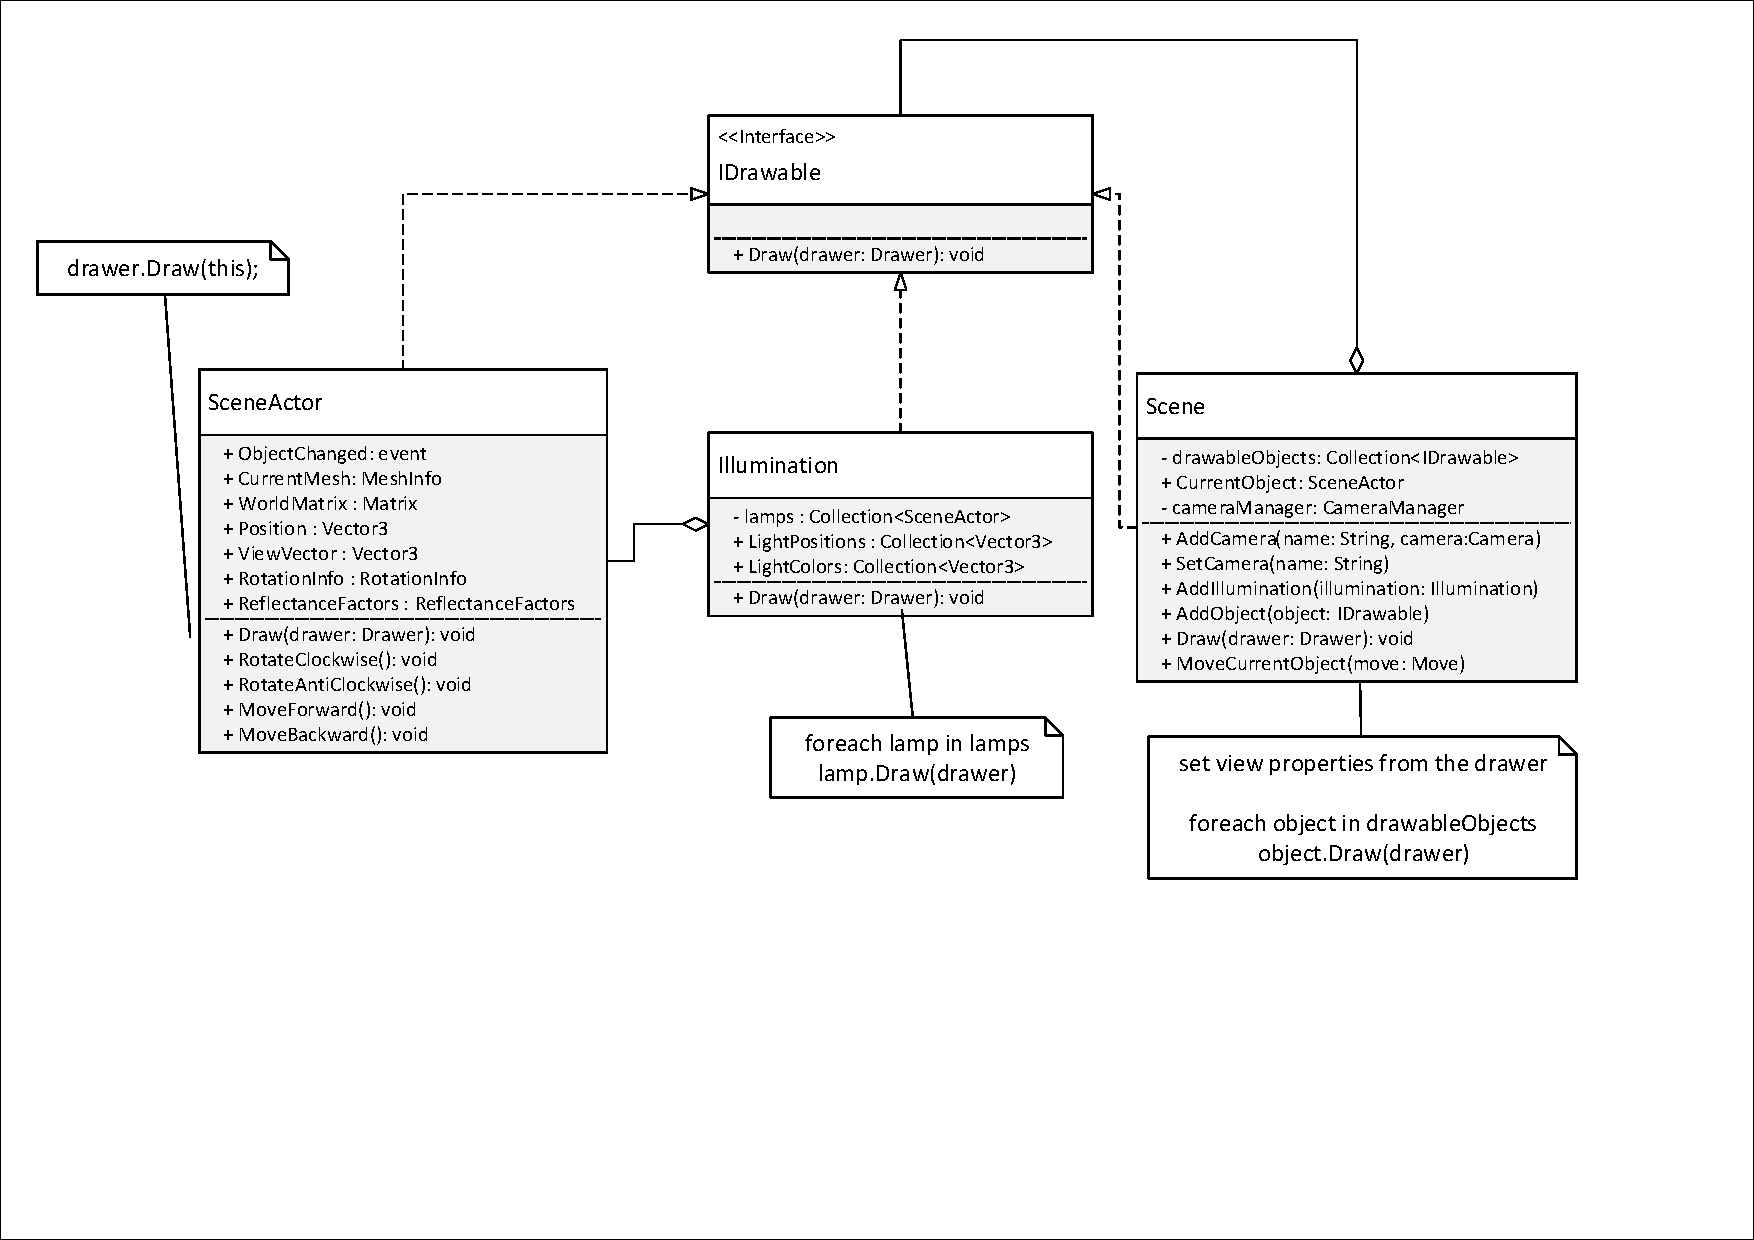
\includegraphics[scale=0.6]{IDrawable.pdf}
\end{figure}
Rysowane mogą być obiekty implementujące interfejs \textit{IDrawable} takie jak: \textit{SceneActor}, \textit{Illumination}, \textit{Scene}.

Klasa \textit{SceneActor} reprezentuje elementarny obiekt, który~może być rysowany. Zawarte są w~niej wszystkie cechy i~właściwości,
związane z~jego wyglądem takie jak: aktualna siatka trójkątów (wewnątrz obiektu klasy \textit{SceneActor} może być wiele siatek trójkątów. Dzięki temu,
możemy symulować animację obiektu), informacje związane z~położeniem, współczynniki pochłaniania/odbicia światła, ,,wektor patrzenia'' (za~jego pomocą
wiemy, jak interpretować ruch obiektu do~przodu/tyłu; ów wektor jest modyfikowany w~momencie wykonywania obrotu obiektu).

Klasa \textit{Illumination} reprezentuje wzór światełek. Składa~się ona z~mniejszych obiektów reprezentujących pojedyncze elemenenty (obiekty klasy \textit{SceneActor}). W~celu optymalizacji wydajności aplikacji, palą się tylko niektóre światełka. Jednakże, nie~jest to zauważalne przez~obserwatora,
gdyż świecące lampki oświetlają pozostałe i~można odnieść wrażenie, że~wszystkie światełka są zapalone. 

Klasa \textit{Scene} enkapsuluje pojedynczą scenę. Zapisane są w~niej referencje do~wszystkich obiektów, które~się na~niej znajdują.
W~szczególności, posiada referencję do~obiektu, którym~użytkownik porusza (\textit{CurrentObject}).
Co~więcej, w~scenie jest zapisana referencja do~,,zarządcy kamer'', który~jest odpowiedzialny za~to, co~użytkownik widzi na~ekranie.
Zarządzanie kamerami zostanie wyjaśnione w~następnym podrozdziale.

Rysowanie zostało zaimplementowane przy~pomocy wzorca projektowego ,,kompozyt'' (obiekty rysowalne są budowane za~pomocą mniejszych
obiektów rysowalnych) i~,,strategia'' (\textit{DrawersManager}) oraz~,,podwójnego rozsyłania'' (\textit{ang. double dispatch}).

\subsubsection{Zarządzanie kamerami}
Zarządzanie kamerami odbywa~się w~podobny sposób do~zarządzania ,,rysownikami''. Mianowicie, za~zarządzanie kamerami odpowiedzialny jest \textit{CameraManager}, która~posiada referencje do~wszystkich aktualnie istniejących kamer i~pamięta obecnie ustawioną kamerę. 
Ponadto, posiada~dwie właściwości -- \textit{ViewMatrix} i~\textit{CameraPosition} odczytywane przy~pomocy odpowiadających publicznych pól aktualnie
ustawionej kamery.  \\ 
\begin{figure}[H]
	\centering 
	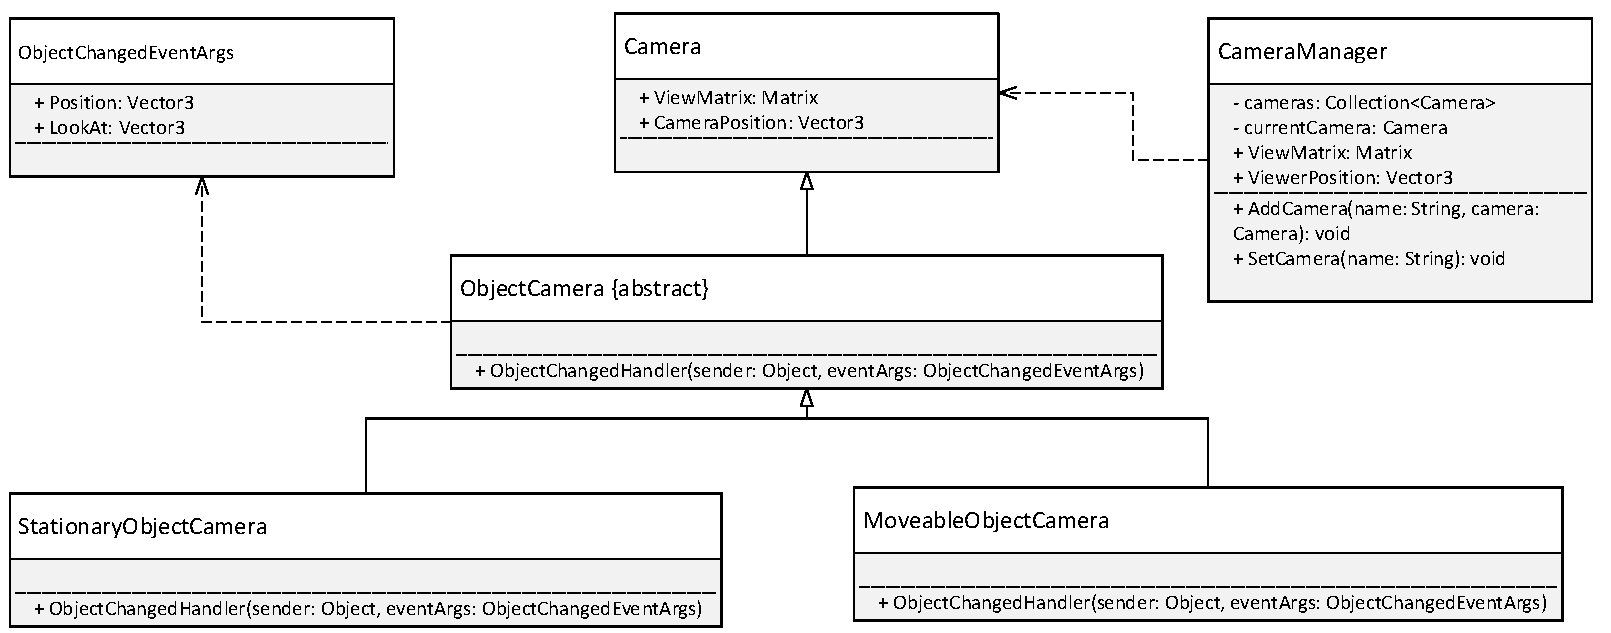
\includegraphics[scale=0.6]{Cameras.pdf}
\end{figure}

W~aplikacji występują 3 rodzaje kamer -- jedna ,,stała'' i~dwie związane z~ruchomym obiektem. Owym~rodzajom odpowiadają odpowiednio klasy
\textit{Camera} i~dwie klasy pochodne abstrakcyjnej klasy \textit{ObjectCamera}.

Jako~że \textit{ObjectCamera} reprezentuje klasę kamer związanych z~ruchomym obiektem, to~konieczne jest powiązanie danej kamery z~konkretnym
obiektem. W~aplikacji realizowane jest to~za pomocą architektury zdarzeń (może to~być również zaimplementowane za~pomocą wzorca projektowego ,,Obserwator'', jeśli~interesujący nas język programowania nie~udostępnia interfejsu zdarzeń). Mianowicie, w~trakcie tworzenia obiektu
kamery (związanej z~obiektem), klasa kamery ,,rejestruje''~się na~otrzymywanie informacji o~zajściu zdarzenia (zdarzenie \textit{ObjectChanged}).
Zatem obiekt ,,obserwowany'' nie~wie przez~kogo jest obserwowany. Owe~zdarzenie jest generowane po~zmianie położenia danego obiektu.

Przed~rozpoczęciem procedury rysowania ustawiane są aktualne dane dotyczące widoku (\textit{ViewMatrix} i~\textit{CameraPosition}) zapisane
w~\textit{CameraManager}.

\section{Dokumentacja końcowa (powykonawcza)}
\subsection{Biblioteki}
Aplikacja została zaimplementowana w~technologii .NET z~pomocą biblioteki graficznej \textit{Monogame}.
\subsection{Instrukcja użycia}
\subsubsection{Sterowanie obiektem}
Sterowanie odbywa~się przy~pomocy strzałek: 
\begin{itemize}
	\item Obrót za pomocą strzałek ,,prawo'' / ,,lewo''
	\item Ruch w~przód/tył za~pomocą strzałek ,,góra'' / ,,dół''
\end{itemize}
\subsubsection{Zmiana modelu oświetlenia}
Dostępne są dwa modele oświetlenia:
\begin{itemize}
	\item Ustawienie modelu Phonga za~pomocą kombinacji klawiszy: \texttt{Alt + P}
	\item Ustawienie modelu Blinna za~pomocą kombinacji klawiszy: \texttt{Alt + B}
\end{itemize}
\subsubsection{Zmiana modelu cieniowania}
Dostępne są trzy modele cieniowania
\begin{itemize}
	\item Ustawienie modelu Phonga za~pomocą kombinacji klawiszy: \texttt{Shift + P}
	\item Ustawienie modelu Gorauda za~pomocą kombinacji klawiszy: \texttt{Shift + G}
	\item Ustawienie cieniowania płaskiego za~pomocą kombinacji klawiszy: \texttt{Shift + F}
\end{itemize}
\subsubsection{Zmiana kamery}
Dostępne są trzy kamery:
\begin{itemize}
	\item Zmiana na~kamerę stałą za~pomocą kombinacji klawiszy: \texttt{Ctrl + C}
	\item Zmiana na~kamerę nieruchomą śledzącą ruchomy obiekt: \texttt{Ctrl + S}
	\item Zmiana na~kamerę ruchomą, patrzącą ,,oczami'' ruchomego obiektu: \texttt{Ctrl + M}
\end{itemize}
\end{document}